\documentclass[12pt]{article}
\usepackage{amsmath}
\usepackage[margin=2.5cm]{geometry}
\usepackage[utf8]{inputenc}
\usepackage{amsfonts}
\usepackage{fancyhdr}
\usepackage{hyperref}
\usepackage{graphicx}
\usepackage{caption}
\usepackage{subcaption}
\usepackage{setspace}
\usepackage{float}
\usepackage{svg}
\setstretch{1.3} 
\usepackage{array}
\usepackage {xcolor}
%...

\usepackage{multirow} % Required for multirows




%...

%\usepackage{csc}% unknown package
\pagestyle{fancy}
\fancyhead[L]{Project of observation of analysis}
\fancyhead[R]{Page \thepage}
\fancypagestyle{firstpage}{%
  \lhead{}
  \rhead{}
}

\begin{document}
\begin{figure*}[!tbp]
  \begin{subfigure}[b]{0.2 \textwidth}
    
\includegraphics[width=\textwidth]{img/uni}
  \end{subfigure}
  \hfill
  \begin{subfigure}[b]{0.25\textwidth}
    
\includegraphics[width=\textwidth]{img/fani}
  \end{subfigure}
\end{figure*}
\begin{center}
\textbf{Project of observation of analysis} \\[1in]
Professor : Dr. Mohmmad Omidalizarandi\\~\\
St : AmirAbbas Saberi
\\[4in]
\textbf{University of Tehran}\\
Jul,14,2023
\end{center}
	\thispagestyle{firstpage}
\newpage
\section{Introduction}

Satellite radar interferometry (InSAR) is a valuable method for measuring the movement of the Earth's surface. However, the conventional approach has limitations due to various error sources, including temporal decorrelation, geometric decorrelation, and atmospheric signal delay. To address these challenges, radar interferometric time series techniques have been developed to mitigate the impact of these errors and estimate deformation history over time.

One such approach is Persistent Scatterer Interferometry (PSI), which relies on the coherent phase history of point scatterers. Since the locations of these scatterers are initially unknown, PSI involves both estimation and detection problems. The estimation and detection processes are complicated by the fact that the phase observations are wrapped within the interval of $[-\pi, +\pi)$, meaning that the coherence of an image pixel in the time domain cannot be directly assessed. Moreover, assumptions about the spatial and temporal smoothness of the deformation signal, represented by a model, are necessary to estimate the unknown phase ambiguities. Therefore, it is important to evaluate both the accuracy of the model used and the actual phase persistence of the pre-selected pixels.

The estimation and detection process must strike a balance between the multiple potential solutions, which depend on the chosen model, and the uncertainty in the noise level of a specific image pixel. This requires a careful approach to minimize false detections and false rejections of Persistent Scatterers (PS).


In this project, we intend to use the data obtained from ascending and descending satellites to monitor the movement of the earth's surface over a period of time for PSI.
The behavior of PSIs can be linear or periodic or both. Its periodicity can be due to seasonal effects. The movement of a point can be defined as a function, and we know that functions can be replaced by Fourier expansion and the expansion coefficients can be obtained, but Fourier expansion also has problems, for example, when there is a data gap, it is not easy to use this expansion method. Another alternative which is derived from the idea of internal multiplication is the LSSA or least square-spectrum analysis method. In this project, this method can be used as a method for these time series data.
\newpage
\section{Least- Squares Spectral Analysis (LSSA)}
Least Squares Spectral Analysis is a powerful method developed at
the University of New Brunswick.

LSSA was first developed by Vaníček (1968, 1971) as an alternative to
the classical Fourier methods.

\begin{itemize}
\item No need to be a stationary signal!
\item Unlike Fourier, gaps and missing data are ok!
\end{itemize}
\subsection{Mathematics of the least-squares spectrum}

Let us consider a discrete time series $f(t_i)$, where $t_i$ is a vector of
observation times and m is the number of data points in the time series. $C_f$ or $Q_f$ : covariance matrix of the the time series. The idea is to approximate $f$ with another function $g$ using the least squares
principle, so that the differences between $f$ and $g$ (the vector of residuals r)
are minimum in the least-squares sense.


\begin{figure}[h!]
    \centering
    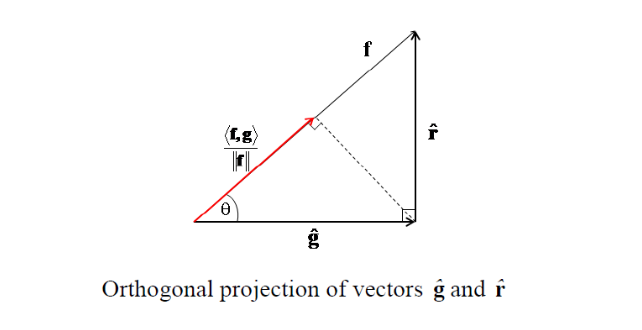
\includegraphics[width=1\linewidth]{img/LSSA}
    \caption{LSSA Concept (Time serise analysis by Zangene)}
    \label{fig:dynamicprogramming}
\end{figure}

from this idea:
\begin{center}
$s = \frac{<f,\hat{g}>/|f|}{|f|} = \frac{f^T C_f^{-1} \hat{g}}{f^T C_f^{-1} f}$
\end{center}
In spectral analysis it is usual to search for periodic signals which can be expressed in
terms of sine and cosine base functions.
\begin{center}
$S(\omega_j) = \frac{y^T Q_y^{-1} A_j \hat{x}_j}{y^T Q_y^{-1} y}$ for $j = 1,2,...,k$
\end{center}
which estimates how much of the wave of cyclic frequency $\omega_j$ contributes to signal.
where $A_j = \begin{bmatrix}
cos(\omega_j t_1) & sin(\omega_j t_1) \\
. & . \\
. & . \\
. & . \\
cos(\omega_j t_m) & sin(\omega_j t_m) \\
\end{bmatrix}
$ in which m is the length of time series. also $\hat{x}_j = (A_j^T Q_y^{-1} A_j)^{-1} A_j^T Q_y^{-1} y$

Note: We call S as the least-squares spectral in percentage $(S(\omega_j)) \in 
(0,1))$.The larger the S (closer to 1) the better is the least-squares fit to the data.
It was shown by Vanicek [1971] that the known constituents (such
as a linear trend) do not have to be removed from time series
before evaluating the spectrum. It speeds the computations up, however, if the least-squares
estimate is removed before the spectrum is evaluated.


\subsection{Least- Squares Spectrum evaluation}
LSSA allows performing statistical testing on the significance of spectral
peaks. This is very important since we need to know which peak is statistically
significant and which one can be suppressed. \\ 
$S(\omega) = {S(\omega_1),S(\omega_2), ...,S(\omega_k)}$ :spectrum 
\begin{center}
$S(\omega_j) =  \begin{cases} 
\leq (1 + \frac{\nu}{2}F_{\nu,2,\alpha})^{-1} : Accept H_0\\
\geq (1 + \frac{\nu}{2}F_{\nu,2,\alpha})^{-1}
: Reject H_0
\end{cases}$
\end{center}
\newpage
\section{Problem Solving}
We have selected the area that includes subsidence and seasonal changes in height according to the figure and we have implemented the LSSA method for them. compared to the accurate estimate on the data.
\begin{figure}[h!]
    \centering
    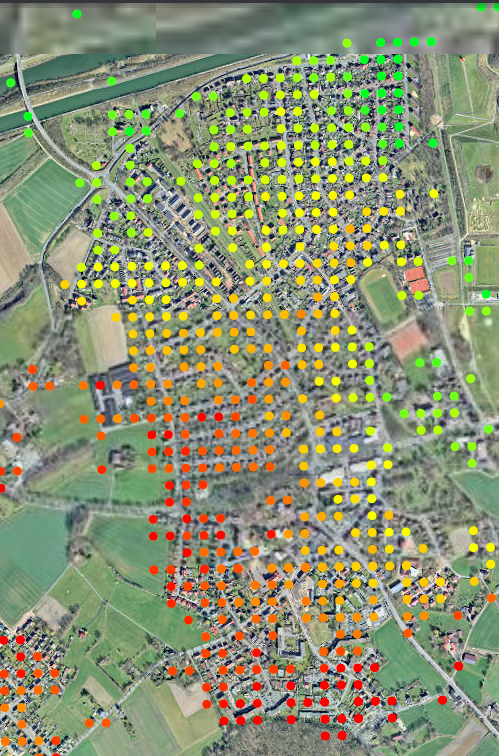
\includegraphics[width=0.3\linewidth]{img/Area}
    \caption{A selected region in Germany}
    \label{fig:dynamicprogramming}
\end{figure}


\begin{figure}[h!]
    \centering
    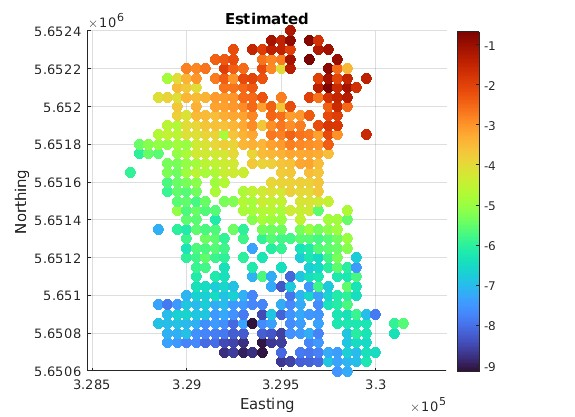
\includegraphics[width=0.6\linewidth]{img/Real}
    \caption{The amount estimated for the subsidence of the area}
    \label{fig:dynamicprogramming}
\end{figure}

\newpage
Estimate output and compare with actual value :
\begin{figure}[h!]
    \centering
    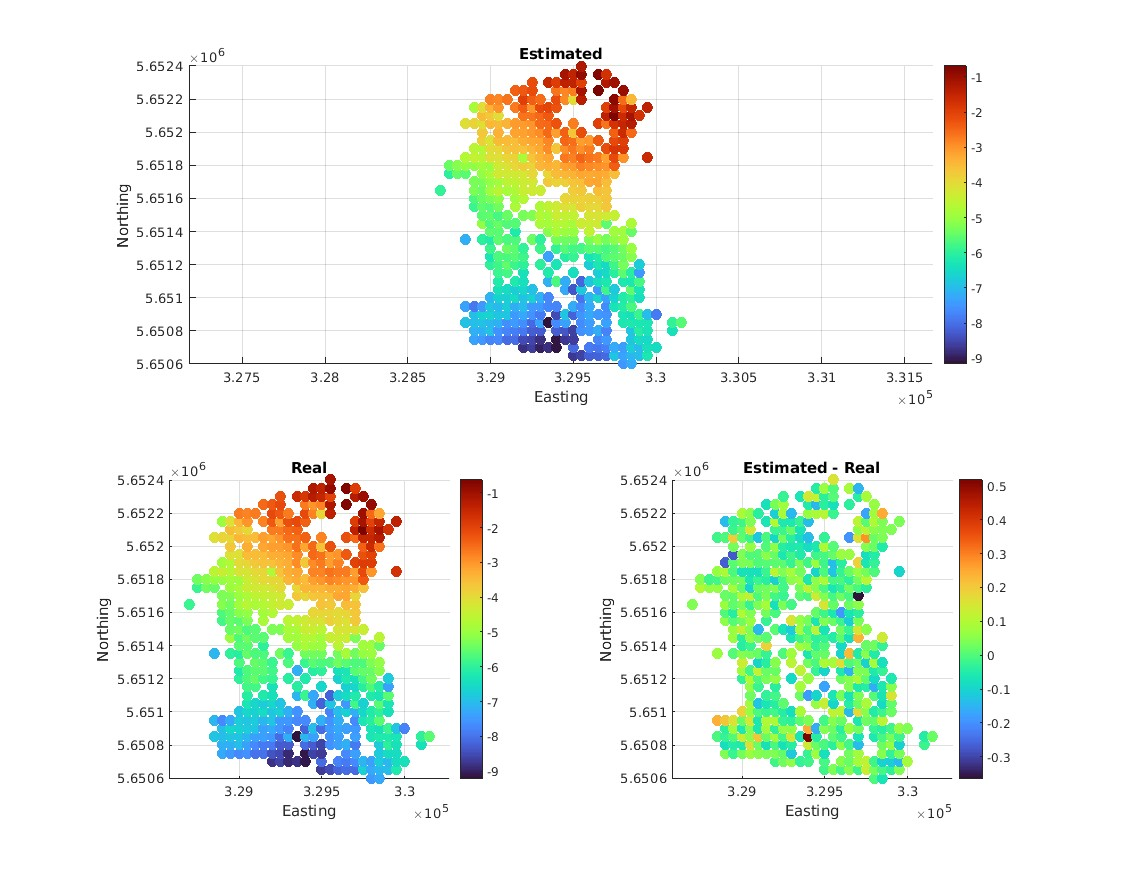
\includegraphics[width=1\linewidth]{img/Result}
    \caption{
The difference between the estimated value and the actual value}
    \label{fig:dynamicprogramming}
\end{figure}


\begin{figure}[h!]
    \centering
    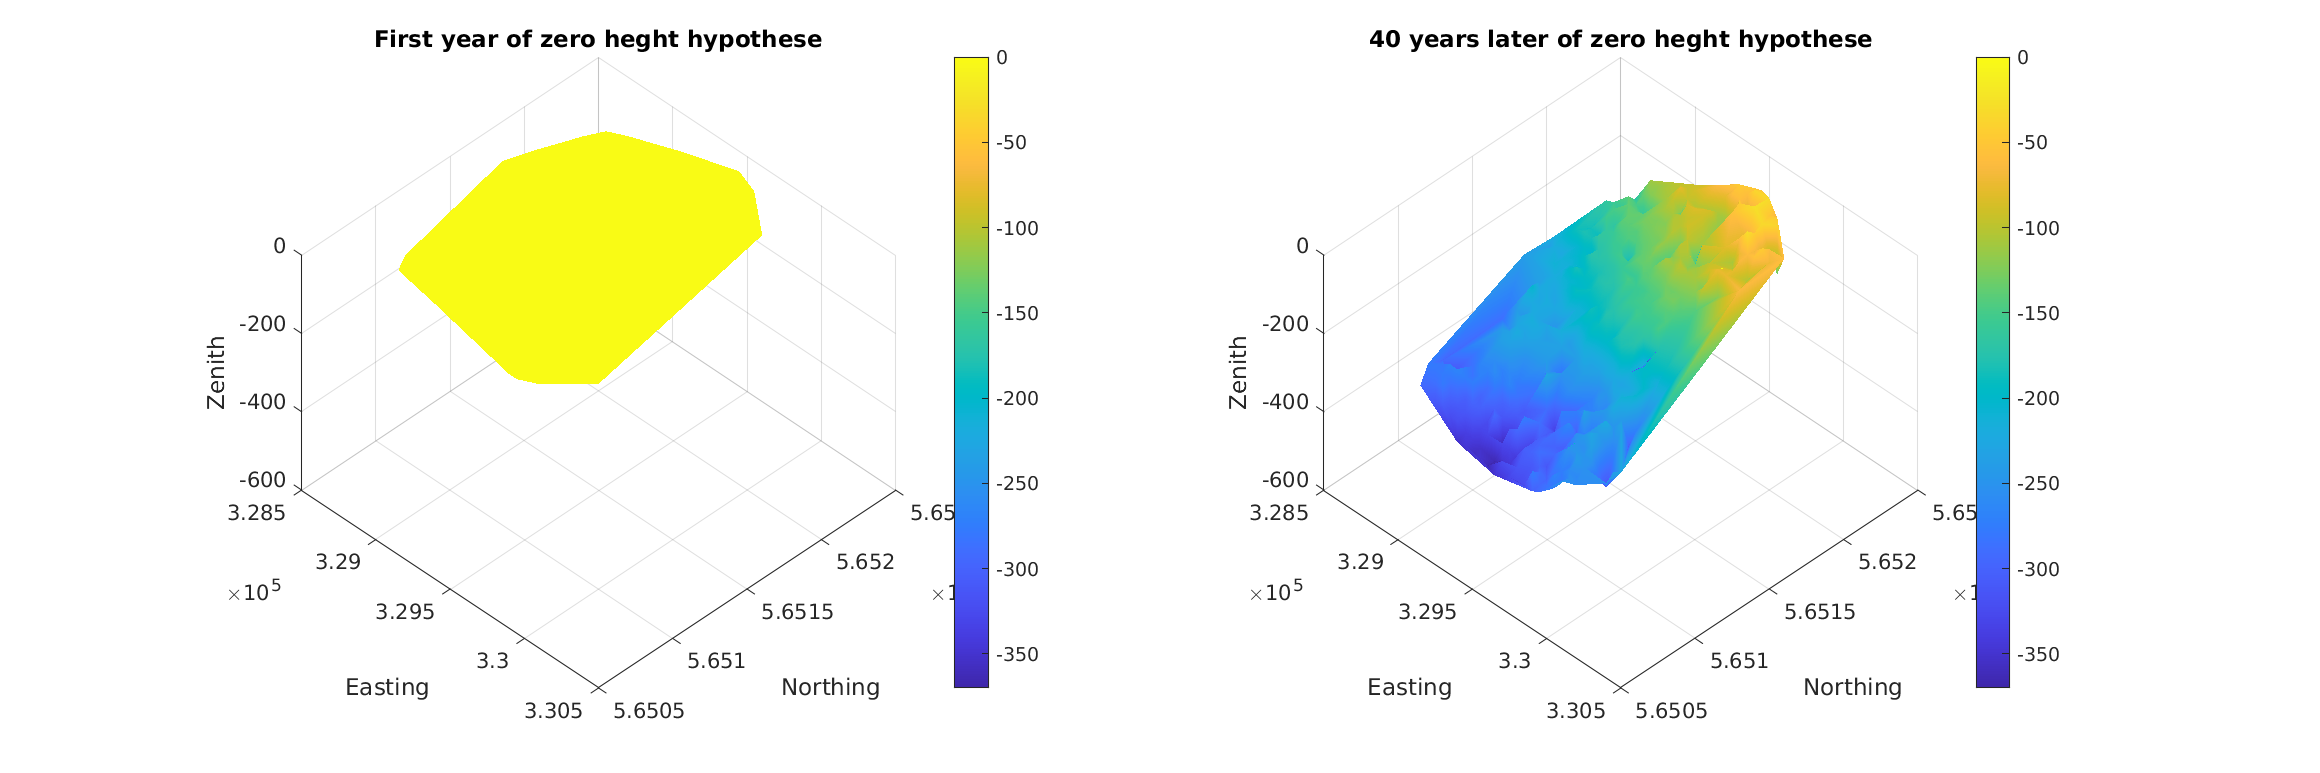
\includegraphics[width=1\linewidth]{img/40}
    \caption{Consider a flat screen and what happens to the screen due to 40 years of Franchest}
    \label{fig:dynamicprogramming}
\end{figure}
\section{Result:}
The resulting subsidence is much greater in the southern part, perhaps the aquifers are drained more in this part
\end{document}



